\chapter{Background}

\section{Early Work in {\IterComp}}

\textbf{Original work in {\IterComp}: single input and offline}

\section{Program Profiling}

\textbf{Basic background about profiling in general}

\section{LLVM Compiler Infrastructure}

LLVM was originally proposed as a \textit{Low-Level Virtual Machine}\footnote{Although LLVM was initially an acronym for Low-Level Virtual Machine, it is now a brand that applies to the whole LLVM umbrella project.}, extending previous work on virtual instruction set architectures~\citep{adve03,lattner04}.
Since then, LLVM has evolved into an umbrella project that comprises a collection of modular and reusable compiler and toolchain technologies.
The main components under the LLVM umbrella is the LLVM intermediate representation (IR) and the LLVM \textit{Core} libraries.

The LLVM compiler infrastructure implements the classical \textit{three-phase compiler} infrastructure, which consists of a frontend, an optimiser, and a backend.
The frontend is responsible for parsing, validating and diagnosing errors in the source code.
This parsed source code is then translated into an intermediate representation, which is the LLVM IR in this case.
The optimiser is responsible for doing a broad variety of transformations, that are usually independent of language and target machine, to improve the code's performance.
%The front end parses source code, checking it for errors, and builds a language-specific Abstract Syntax Tree (AST) to represent the input code. The AST is optionally converted to a new representation for optimization, and the optimizer and back end are run on the code.
%The optimizer is responsible for doing a broad variety of transformations to try to improve the code's running time, such as eliminating redundant computations, and is usually more or less independent of language and target.
The backend, also known as the code generator, then translates the code from the intermediate representation onto the target instruction set.
It is common for the backend to also perform some low-level optimisations that take advantage of unusual features of the supported architecture.
%Common parts of a compiler backend include instruction selection, register allocation, and instruction scheduling.

\begin{figure}[h]
  \centering
  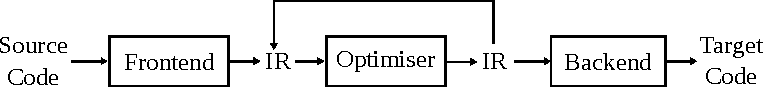
\includegraphics[scale=0.9]{figs/3-phase-compiler.pdf}
  \caption{Overview of the three-phase compiler infrastructure.}
  \label{fig:3-phase-compiler}
\end{figure}

%This IR is optionally fed through a series of analysis and optimization passes which improve the code, then is sent into a code generator to produce native machine code, as shown in Figure 11.3.
%This is a very straightforward implementation of the three-phase design, but this simple description glosses over some of the power and flexibility that the LLVM architecture derives from LLVM IR.

%The most important aspect of its design is the LLVM Intermediate Representation (IR), which is the form it uses to represent code in the compiler.
%LLVM IR is designed to host mid-level analyses and transformations that you find in the optimizer section of a compiler.
%It was designed with many specific goals in mind, including supporting lightweight runtime optimizations, interprocedural optimizations, whole program analysis, and aggressive restructuring transformations, etc.

%Like a real RISC instruction set, it supports linear sequences of simple instructions like add, subtract, compare, and branch.

LLVM IR is a low-level RISC-like virtual instruction set.
It differs from other intermediate representations (e.g. GCC's GENERICS or the most recent GCC's GIMPLE) as it is defined as a first class language with well-defined semantics.
Beyond being implemented as a language, LLVM IR is actually defined in three isomorphic forms: the textual format above, an in-memory data structure inspected and modified by optimizations themselves, and an efficient and dense on-disk binary "bitcode" format.
The LLVM Project also provides tools to convert the on-disk format from text to binary: llvm-as assembles the textual .ll file into a .bc file containing the bitcode goop and llvm-dis turns a .bc file into a .ll file.


Unlike most RISC instruction sets, LLVM is strongly typed with a simple language-independent type system.
LLVM's type system can be used to implement data types and operations from high-level languages exposing their implementation behaviour to all stages of optimisation.
This type system includes the type information used by sophisticated techniques, such as algorithms for pointer analysis, dependence analysis, and data transformations.
LLVM also offers instructions for performing type conversions and low-level address arithmetic while preserving type information.
Furthermore, LLVM IR also differs from RISC instruction sets as some details of the machine are abstracted away.
For example, the calling convention is abstracted through call and ret instructions and explicit arguments.
Another significant difference from machine code is that the LLVM IR doesn't use a fixed set of named registers, it uses an infinite set of temporaries named with a \% character.

In addition to type information, LLVM IR also provides other high-level information that are useful for effectively performing several code analysis and transformations.
This includes explicit control flow graphs (CFG) and an explicit dataflow representation, by means of the infinite register set in \textit{static single assignment} (SSA) form~\citep{}.

SSA FORM

\textbf{Another difference between LLVM and GCC:}

In particular, LLVM IR is both well specified and the only interface to the optimizer.
This property means that all you need to know to write a front end for LLVM is what LLVM IR is, how it works, and the invariants it expects.
Since LLVM IR has a first-class textual form, it is both possible and reasonable to build a front end that outputs LLVM IR as text, then uses Unix pipes to send it through the optimizer sequence and code generator of your choice.

It might be surprising, but this is actually a pretty novel property to LLVM and one of the major reasons for its success in a broad range of different applications.
Even the widely successful and relatively well-architected GCC compiler does not have this property: its GIMPLE mid-level representation is not a self-contained representation.
As a simple example, when the GCC code generator goes to emit DWARF debug information, it reaches back and walks the source level "tree" form.
GIMPLE itself uses a "tuple" representation for the operations in the code, but (at least as of GCC 4.5) still represents operands as references back to the source level tree form.

The implications of this are that front-end authors need to know and produce GCC's tree data structures as well as GIMPLE to write a GCC front end.
The GCC back end has similar problems, so they also need to know bits and pieces of how the RTL back end works as well.
Finally, GCC doesn't have a way to dump out "everything representing my code", or a way to read and write GIMPLE (and the related data structures that form the representation of the code) in text form. The result is that it is relatively hard to experiment with GCC, and therefore it has relatively few front ends.


\textbf{IR, what is a Basic Block, SSA Form}
